\chapter{Campus Universitario}
\label{chap:Campus Universitario}

La Universidad Mayor de San Simón fue fundada mediante ley de 5 de noviembre de 1832 por el Mariscal Andrés de Santa Cruz. La misma ley dispuso la creación y funcionamiento de una Academia de Practicantes Juristas, con la que, en realidad, se inicia la Facultad de Derecho, y hasta la fecha la Universidad cuenta con 12 Facultades de las cuales 7 se encuentran dentro del campus. \cite{umss_history}

Actualmente dentro la página de la Universidad se puede encontrar un ``Mapa Universitario'', el cual se puede apreciar en la figura \ref{fig:mapa_old}, este mapa consiste en una vista del campus universitario como un todo dentro del plano de la ciudad de Cochabamba, la misma página cuenta con la sección ``Paseo Virtual'' la cual lamentablemente no muestra nada.\\

\begin{figure}[H]
  \begin{center}
    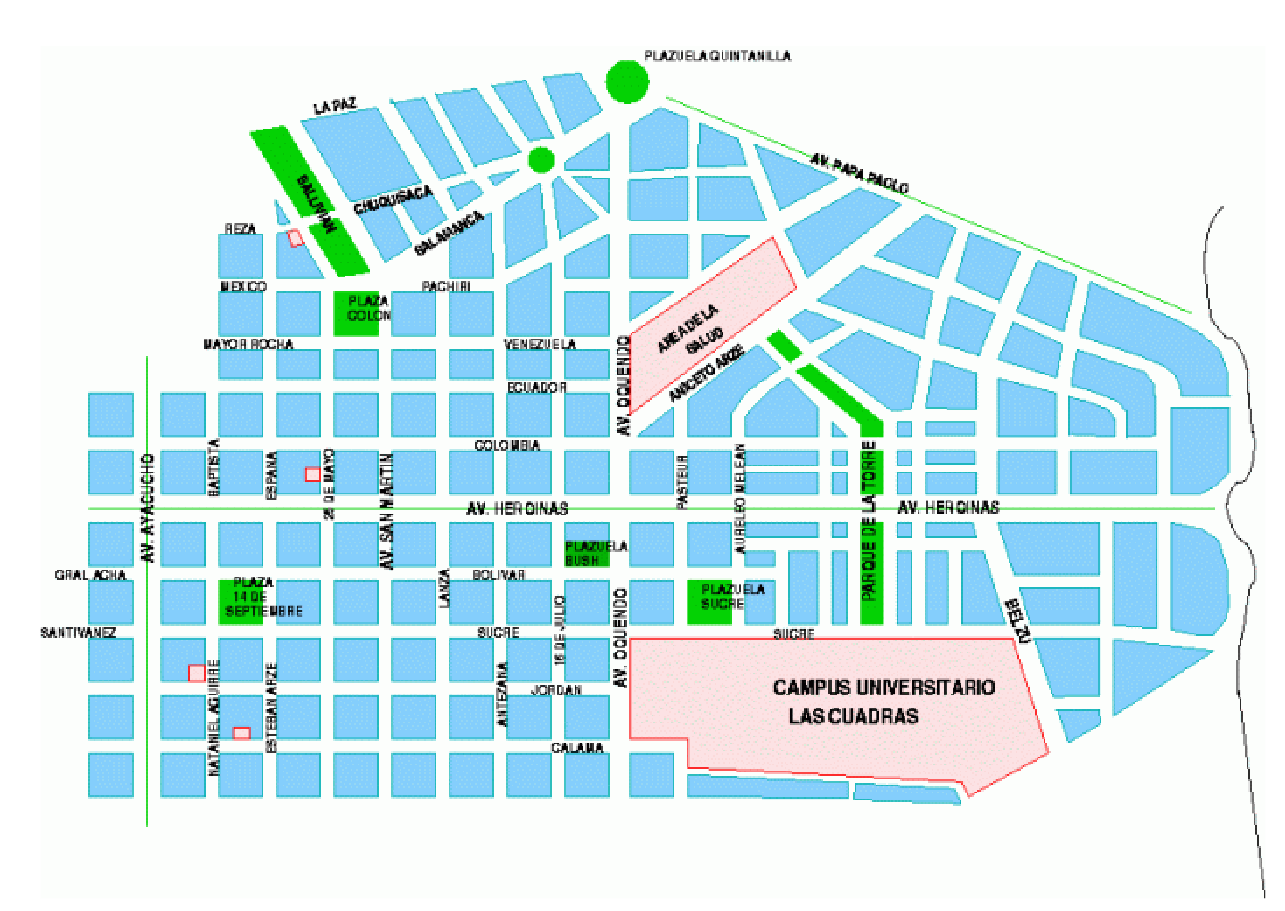
\includegraphics[width=0.75\textwidth]{mapa_old}
    \caption{Mapa universitario}
    \label{fig:mapa_old}
    \caption*{Fuente: \cite{umss_mapa}}
  \end{center}
\end{figure}


% Como personas que usamos los predios del campus ya sea como estudiantes, docentes o visitantes, todos necesitamos contar con un mapa más actualizado del campus universitario.\\
Los estudiantes, docentes y visitantes que usan y circulan dentro de los predios del campus, necesitan contar con un mapa más actualizado


Actualmente dentro del campus universitario ``Las Cuadras'' se puede encontrar las siguientes sectores:

\begin{enumerate}
\item FACH - Facultad de Arquitectura y Ciencias del Hábitat
% Dirección: Calle Jordán Interior
% Teléfonos: 4255730-4231172

\item FCJyP - Facultad de Ciencias Jurídicas y Políticas
% Dirección: Campus Central: Av. Oquendo esq Sucre
% Teléfonos: 591-4-4227509

\item FACES - Facultad de Ciencias Económicas
% Dirección: Edificio Prototipo I - Final Calama Este Campus Universitario
% Teléfonos: 4540245 - 4540248 - 4540261 FAX: 4540257


\item FHCE - Facultad de Humanidades y Ciencias de la Educación
% Dirección: Plaza Sucre acera Sud
% Teléfonos: 591-4-4544102

\item FCyT - Facultad de Ciencias y Tecnología
% Dirección: Calle Sucre y parque la Torre
% Teléfonos: 591-4-4231765

\item Multiacademico
\item Complejo Deportivo


\end{enumerate}

La Universidad cuenta con Aulas numeradas hasta el 758, repartidas entre todas las facultades y hasta para un estudiante que pasa gran parte de su tiempo dentro del campus es difícil encontrar un lugar cuando no se sabe su locación exacta, entonces para un visitante ocasional esto puede llegar a ser un gran problema.\\

Pero aparte de Aulas también se encuentra del campus, oficinas administrativas, centros de estudiantes, snacks, etc. por lo que conocer con exactitud la locación de un lugar es de gran importancia para no extraviarse dentro del campus universitario.\\


\begin{figure}[H]
  \begin{center}
    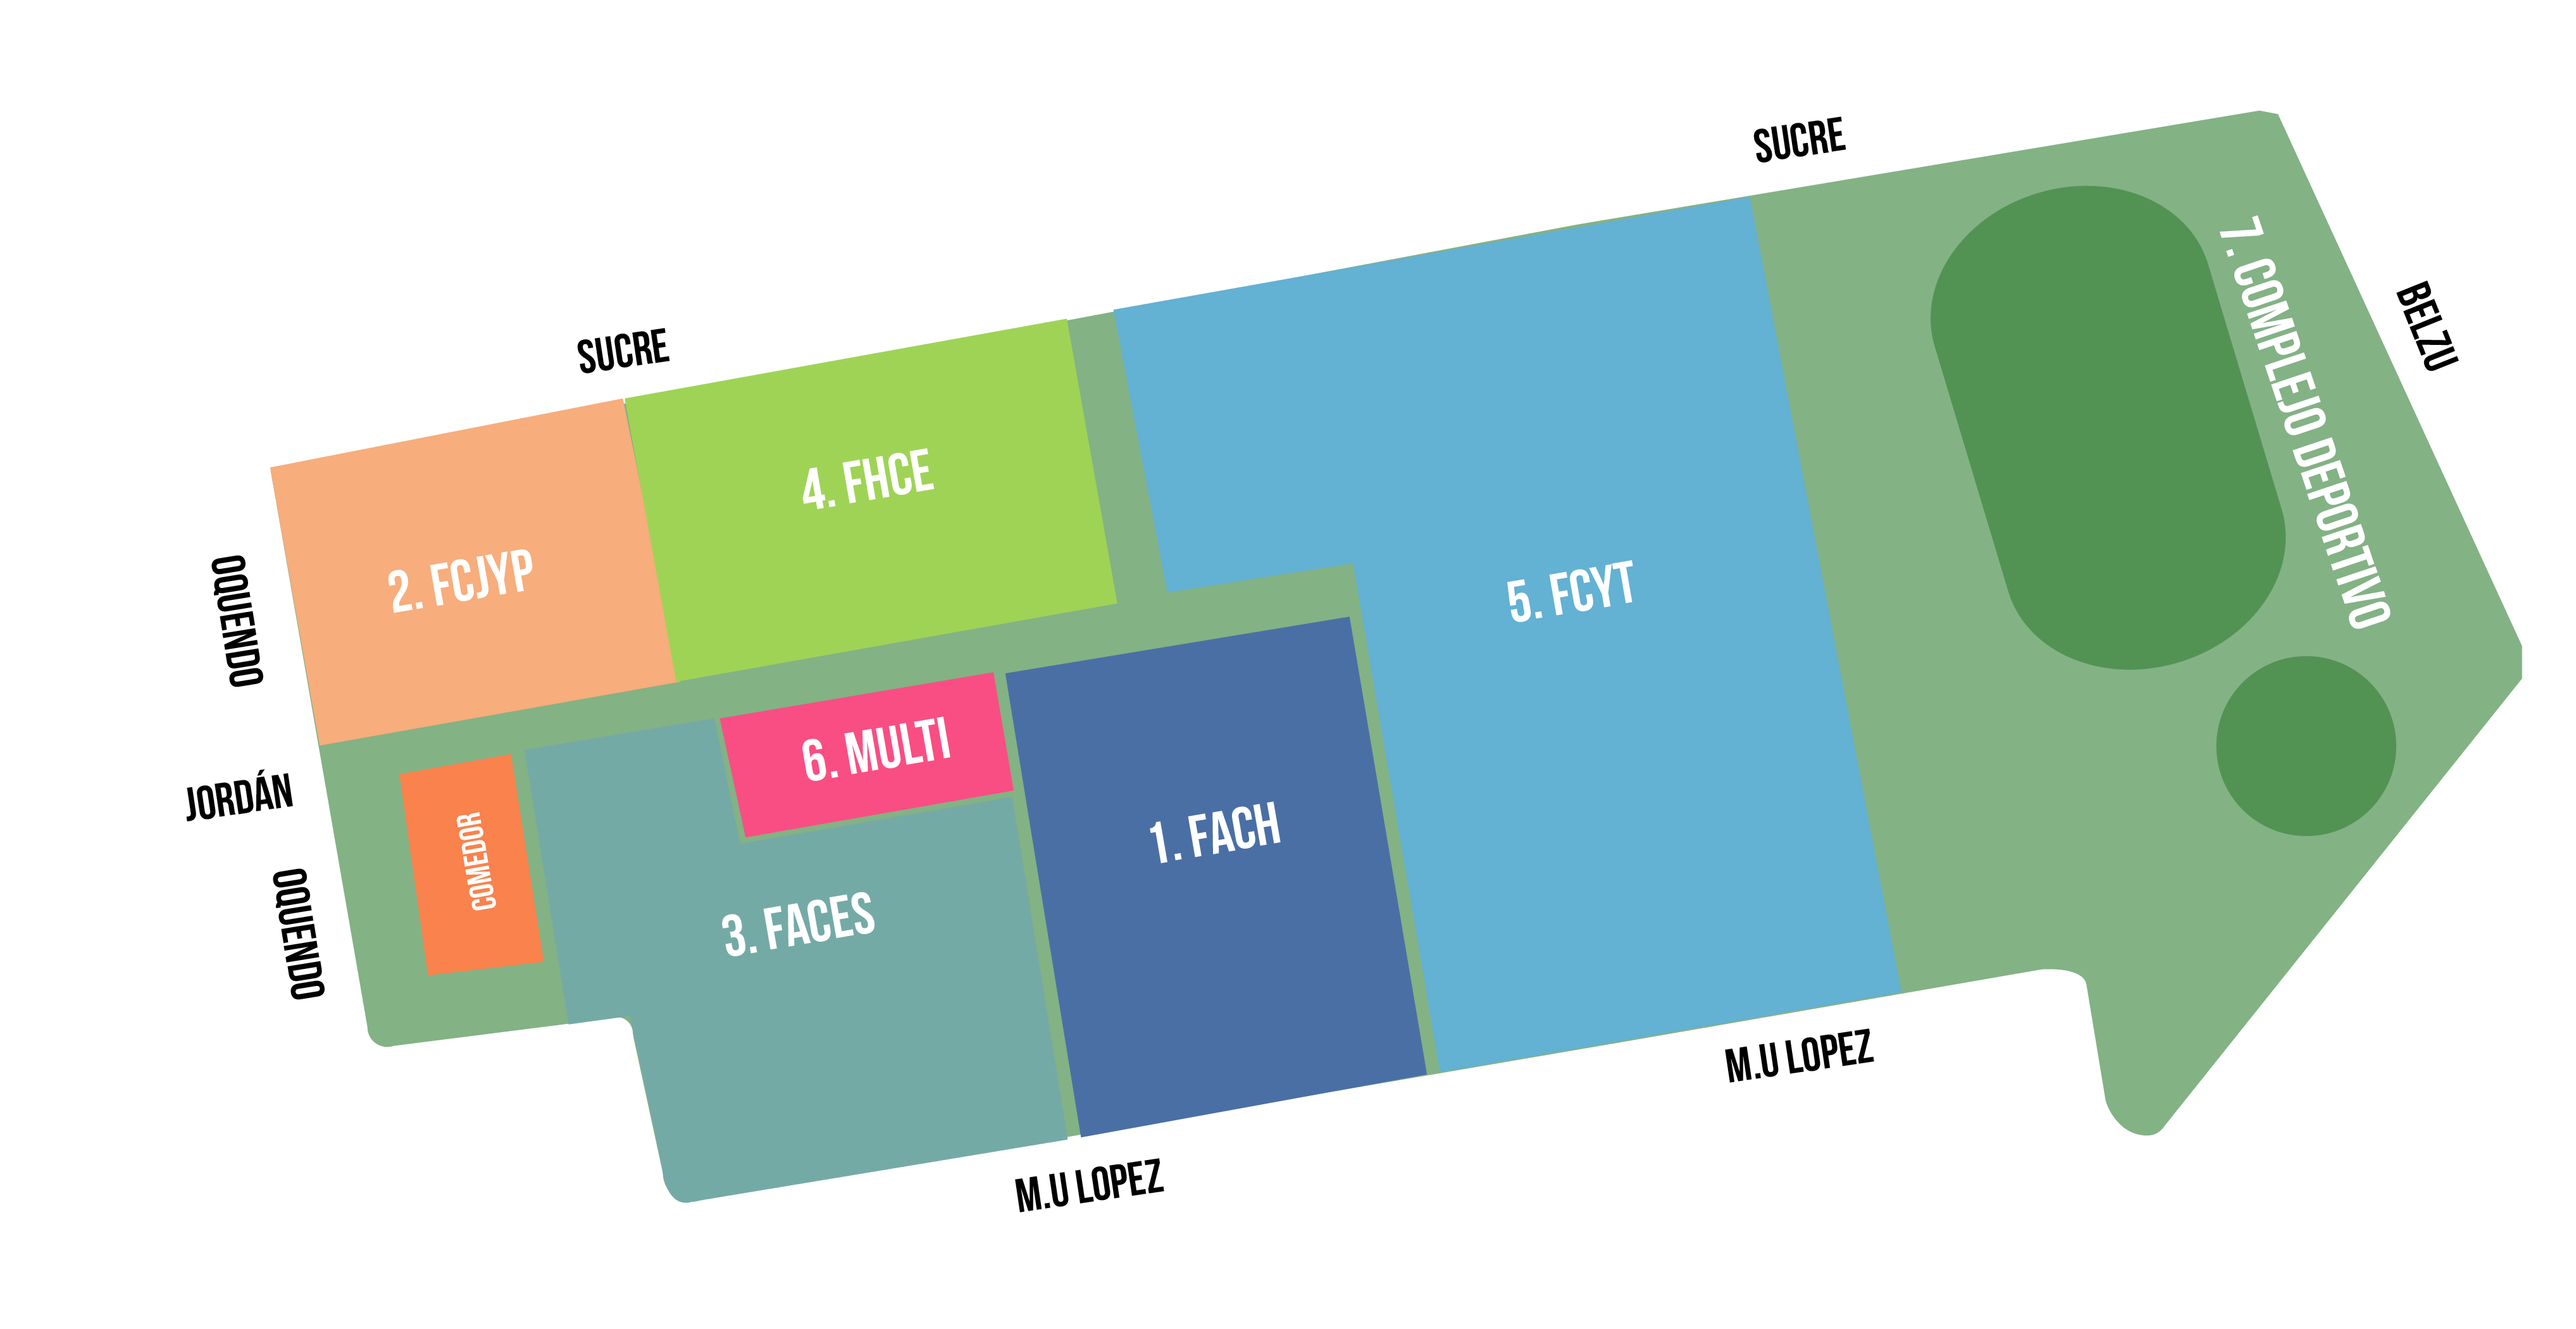
\includegraphics[width=1\textwidth]{mapa_new}
    \caption{Facultades dentro del Campus}
    \label{fig:mapa_new}
    \caption*{Fuente: Elaboración propia}

  \end{center}
\end{figure}


En la figura \ref{fig:mapa_new} se puede apreciar a grandes rasgos la distribución de las facultades dentro del campus, el mapa sirve para dar una idea de la ubicación de las facultades y edificios administrativos, los cuales son detallados a continuación.

\section{Facultad de Arquitectura y Ciencias del Hábitat}
\label{sec:facultad_arquitectura}

% Dirección: Calle Jordán Interior
% FACH - Facultad de Arquitectura y Ciencias del Hábitat
    La Facultad de Arquitectura y Ciencias del Hábitat colinda con la calle M. U. Lopez, dentro de los predios del campus Universitario se halla entre las facultades de Economía hacia el Sur-Este y con la facultad de Tecnología hacia el Nor-Oeste, en la figura \ref{fig:fac_arqui} se puede apreciar la facultad con las aulas y oficinas que cuenta en su interior.\\

    \begin{figure}[H]
     \begin{center}
       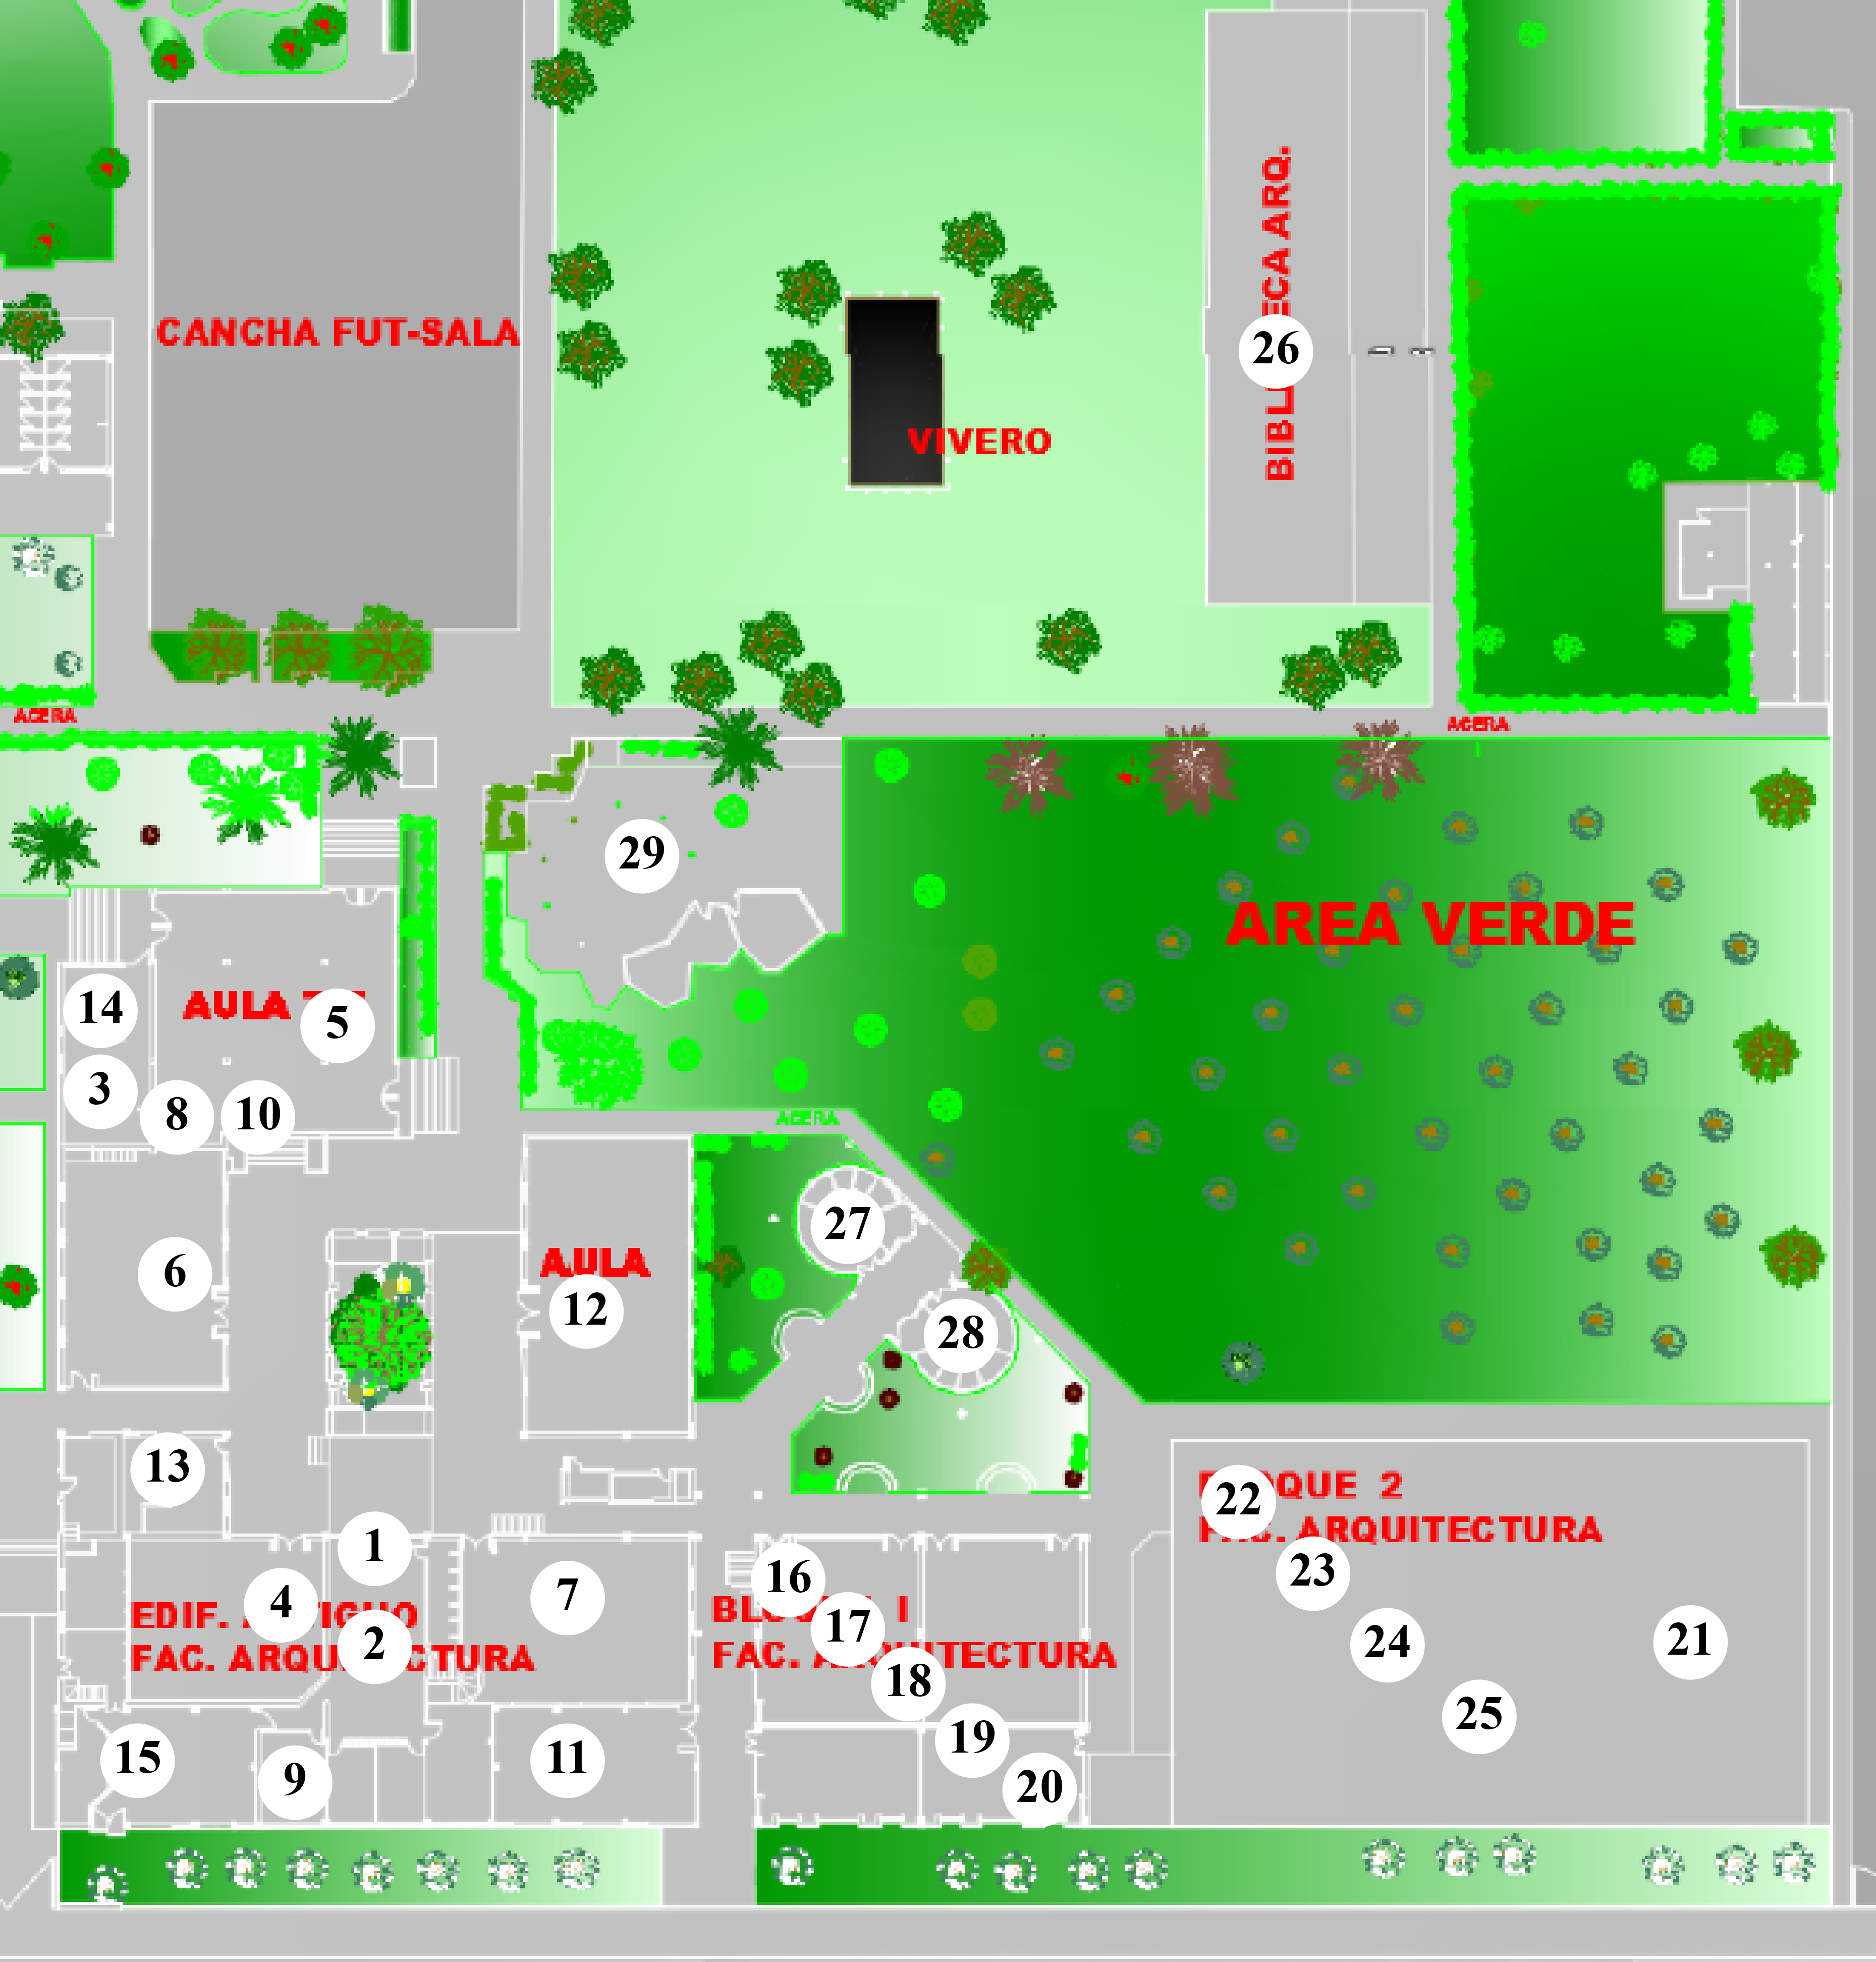
\includegraphics[width=0.8\textwidth]{fac_arquitectura}
       \caption{Facultad de Arquitectura - UMSS}
       \label{fig:fac_arqui}
       \caption*{Fuente: Departamento Infraestructura - UMSS}
     \end{center}
    \end{figure}

    % % \begin{table}
%   \begin{center}
    \begin{longtable}{ c  X }
      \toprule
        \textbf{Punto} &
        \textbf{Detalle}\\

      \midrule
      \endhead

  \textbf{1}
  &
  Decanato FACH
  \\

  \textbf{2}
  &
  Dirección Carrera Arquitectura
  \\

  \textbf{3}
  &
  Dirección Carrera Turismo
  \\

  \textbf{4}
  &
  Asociación Docente de Arquitectura
  \\

\textbf{5}
&
Aula 701
\\

\textbf{6}
&
Aula 702
\\

\textbf{7}
&
Aula 703
\\

\textbf{8}
&
Aula 704
\\

\textbf{9}
&
Aula 705
\\

\textbf{10}
&
Aula 706
\\

\textbf{11}
&
Aula 707
\\

% \textbf{12}
% &
% Aula 708*
% \\

\textbf{12}
&
Aula 709
\\


\textbf{13}
&
Centro de Estudiantes de Arquitectura
\\

\textbf{14}
&
Centro de Estudiantes de Turismo
\\


\textbf{15}
&
Laboratorio de Arquitectura
\\

\textbf{16}
&
Planta Baja - Aulas: 720, 721, 722, 723
\\

\textbf{17}
&
1{\tiny er} Piso - Aulas: 724, 725
\\

\textbf{18}
&
2{\tiny do} Piso - Aulas: 726, 727
\\


\textbf{19}
&
3{\tiny er} Piso - Aulas: 728. 729
\\



\textbf{20}
&
4{\tiny to} Piso - Direccion de Formacion Continua Grado y Postgrado FACH
\\



\textbf{21}
&
Planta Baja - Auditorio ``M.Sc. Arq. Brownie Mostajo Medinaceli''
\\



\textbf{22}
&
1{\tiny er} Piso - Aulas: 740, 741, 742, 743
\\




\textbf{23}
&
2{\tiny do} Piso - Aulas: 745, 746, 747, 748
\\




\textbf{24}
&
3{\tiny er} Piso - Aulas: 750, 751, 752, 753
\\

\textbf{25}
&
4{\tiny to} Piso - Aulas: 755, 756, 757, 758
\\


\textbf{26}
&
Biblioteca FACH
\\

\textbf{27}
&
Aula 729
\\

\textbf{28}
&
EDAV - Estudio de Artes Visuales
\\

\textbf{29}
&
Snack Arquitectura
\\

\textbf{A30}
&
2{\tiny do} Piso - Aulas: 760, 761, 762, 763 - Ver en el mapa del Multiacademico, figura \ref{fig:multiacademico}
\\

\textbf{A31}
&
Aulas: TODO* - Ver en el mapa de Tecnología, figura \ref{fig:fac_tecno}
\\


      \bottomrule
      \caption{Locaciones de la Fac. Arquitectura}
      \label{tab:lugares_arquitectura}
    \end{longtable}
%   \end{center}
% \end{table}

    \LTXtable{0.8\textwidth}{facultades/arquitectura}



 \section{Facultad de Ciencias Jurídicas y Políticas}
 \label{sec:facultad_derecho}

 % La facultad de Derecho cuenta con alrededor de 178 vértices y 88 aristas, está ubicada al nor-oeste del Campus Universitario, en la esquina de la calle Oquendo y Sucre, dentro del campus colinda con la facultad de Humanidades hacia el Nor-Este y hacia el Sur-Oeste está la facultad de Economía.

 Generalmente conocida como ``Facultad de Derecho'' se encuentra al nor-oeste del Campus Universitario, en la Av. Oquendo esquina Sucre. En la figura \ref{fig:fac_derecho} se puede ver las locación de los lugares que se puede encontrar dentro de esta facultad. \\

 \begin{figure}[H]
   \begin{center}
     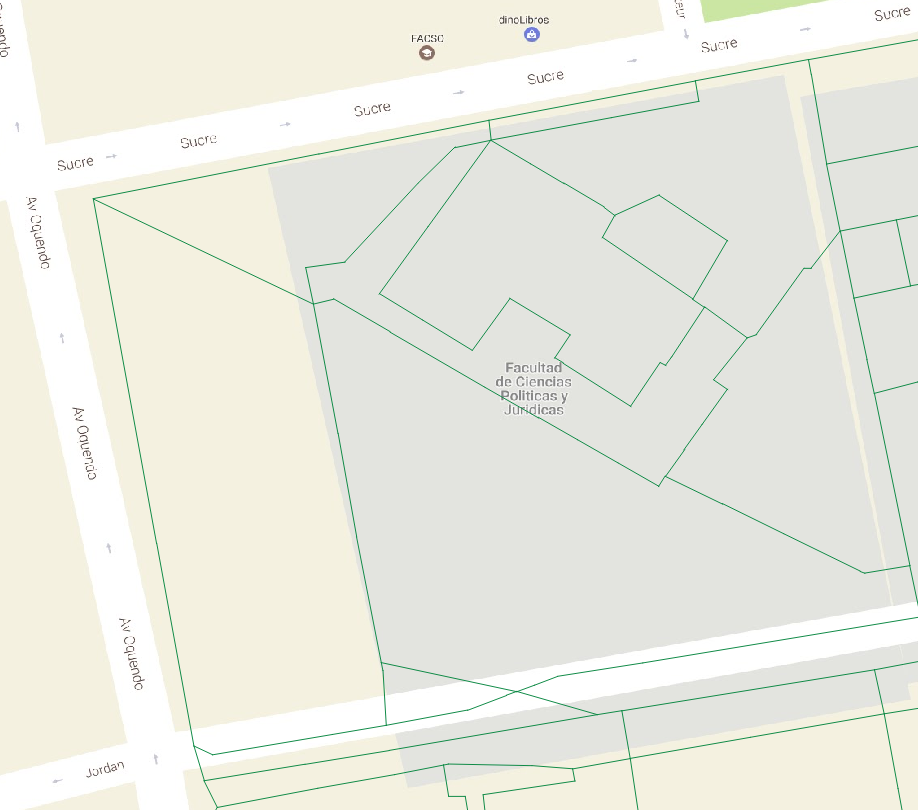
\includegraphics[width=0.8\textwidth]{fac_derecho}
     \caption{Facultad de Derecho - UMSS}
     \label{fig:fac_derecho}
     \caption*{Fuente: Departamento Infraestructura - UMSS}

   \end{center}
 \end{figure}

 \LTXtable{0.8\textwidth}{facultades/derecho}
 % \begin{table}[H]
  \begin{center}
    \begin{tabularx}{\textwidth}{ c  X }
      \toprule
        \textbf{Punto} &
        \textbf{Detalle}\\

      \midrule
        \textbf{1}
        &
        Centro de Estudiantes de Derecho
        \\

      \addlinespace
      \textbf{2}
      &
      1{\tiny er} Piso - Aula PP1, Aula PP2, Aula PP3, Aula PP4, Aula PP5, Aula PP6
      \\

      \addlinespace
      \textbf{3}
      &
      2{\tiny do} Piso - Aula SP1, Aula SP2, Aula SP3, Aula SP4, Aula SP5
      \\

      \addlinespace
      \textbf{4}
      &
      3{\tiny er} Piso - Carrera de Ciencia Politica
      \\

      \addlinespace
      \textbf{5}
      &
      3{\tiny er} Piso - Aula TP1, Aula TP2, Aula TP3, Aula TP4, Aula TP5
      \\

      \addlinespace
      \textbf{6}
      &
      3\text{\tiny er} Piso - Salon Auditorio ``Lic. Orlando Mercado Camacho''
      \\


      \addlinespace
      \textbf{7}
      &
      4{\tiny to} Piso - Aula CP1, Aula CP2, Aula CP3, Aula CP4, Aula CP5
      \\

      \addlinespace
      \textbf{8}
      &
      5{\tiny to} Piso - Aula QP1, Aula QP2, Aula QP3, Aula QP4, Aula QP5, Aula QP6
      \\

      \addlinespace
      \textbf{9}
      &
      Aula BA1
      \\

      \addlinespace
      \textbf{10}
      &
      Oficina Educativa Virtual Facultativa
      \\

      \addlinespace
      \textbf{11}
      &
      Full
      \\

      \addlinespace
      \textbf{12}
      &
      SITUMSS - Sindicato Trabajadores UMSS
      \\

      \addlinespace
      \textbf{13}
      &
      Snack Derecho
      \\

      \addlinespace
      \textbf{14}
      &
      Torre Fotos UMSS
      \\


      \bottomrule
    \end{tabularx}
    \caption{Locaciones de la Fac. Derecho}
    \label{tab:lugares_derecho}
  \end{center}
\end{table}




 % En la figura \ref{fig:fac_derecho} se puede observar en la línea verde los caminos o rutas dentro de la facultad de derecho de la UMSS, proyectada sobre el mapa de Google Maps, para lograr esta representación se utilizó QGIS ya que la información geográfica de la ruta está contenida en un archivo shapefile y el mapa se lo obtiene usando el API de Google Maps gracias al plugin de QGIS, \emph{QuickMapServices}.

 % \footnote{http://nextgis.com/blog/quickmapservices/}.




\section{Facultad de Ciencias Económicas}
\label{sec:facultad_economia}

      % Dirección: Edificio Prototipo I - Final Calama Este Campus Universitario
      La Facultad de Ciencias Económicas o comúnmente conocida como ``Facultad de Economía''
      colinda con las calles Oquendo y M. U. López, dentro del campus al Nor-Este se encuentra la facultad de Arquitectura y al Nor-Oeste la facultad de Derecho, tal como se puede apreciar en la figura \ref{fig:fac_economia}.

      \begin{figure}[H]
       \begin{center}
         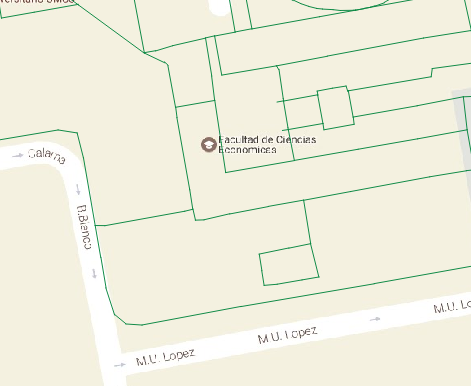
\includegraphics[width=1\textwidth]{fac_economia}
         \caption{Facultad de Economía - UMSS}
         \label{fig:fac_economia}
         \caption*{Fuente: Departamento Infraestructura - UMSS}

       \end{center}
      \end{figure}


      \LTXtable{0.8\textwidth}{facultades/economia}




\section{Facultad de Humanidades y Ciencias de la Educación}
\label{sec:facultad_humanidades}

La entrada a la facultad de Humanidades se lo encuentra sobre la calle Sucre en frente de la \emph{Plaza Sucre} acera Sud, en la figura \ref{fig:fac_humanidades} se puede apreciar la \emph{FHCE} dentro del campus Universitario y en la tabla \ref{tab:lugares_humanidades} se puede ver el detalle de los lugares que se pueden ubicar dentro de la facultad de Humanidades y Ciencias de la Educación.

\begin{figure}[H]
 \begin{center}
   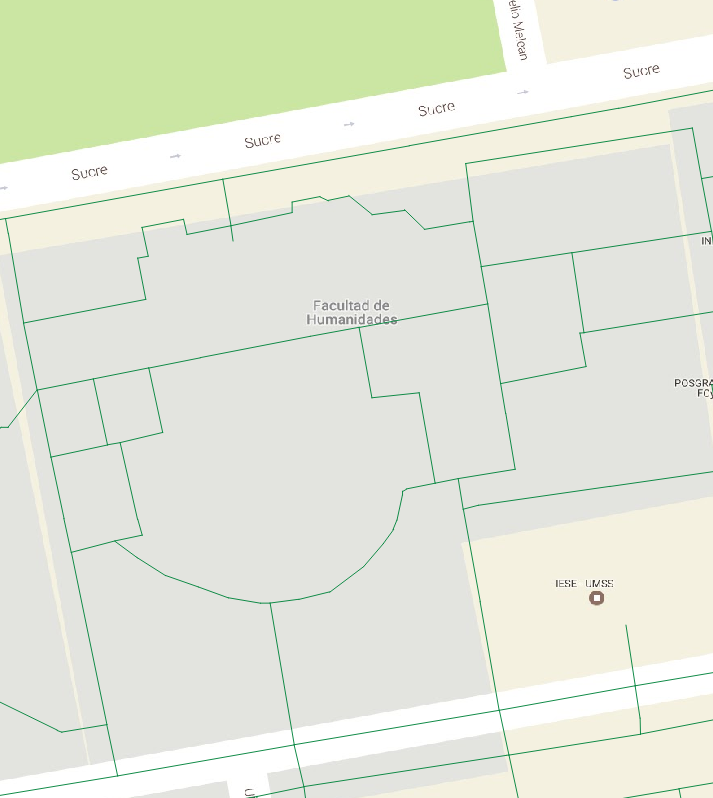
\includegraphics[width=0.75\textwidth]{fac_humanidades}
   \caption{Facultad de Humanidades - UMSS}
   \label{fig:fac_humanidades}
   \caption*{Fuente: Departamento Infraestructura - UMSS}
 \end{center}
\end{figure}

\LTXtable{0.8\textwidth}{facultades/humanidades}



\section{Facultad de Ciencias y Tecnología}
\label{sec:facultad_tecnologia}

Comúnmente conocida como ``facultad de Tecnología'',  se encuentra en el sector Nor-Este dentro del campus Universitario, se puede encontrar una entrada a la facultad de tecnología sobre la calle  al frente del parque \emph{la Torre} y otra entrada sobre la calle MU Lopez debajo de los edificios nuevos de tecnología, dentro del campus Universitario colinda con las facultades de Arquitectura y Humanidades que se encuentran hacia el Sur-Este y Sur-Oeste correspondientemente, en la siguiente figura \ref{fig:fac_tecno} se puede apreciar la facultad de Tecnología.

\begin{figure}[H]
 \begin{center}
   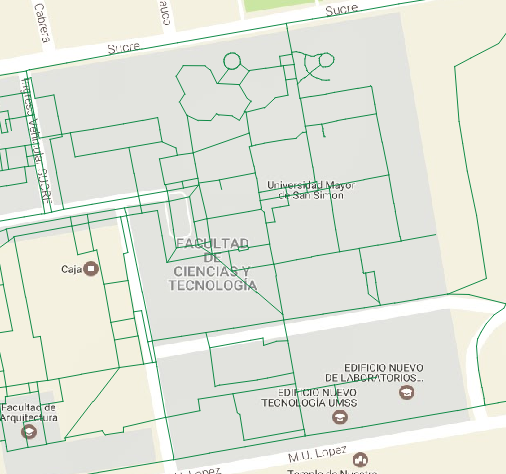
\includegraphics[width=0.9\textwidth]{fac_tecno}
   \caption{Facultad de Tecnología - UMSS}
   \label{fig:fac_tecno}
   \caption*{Fuente: Departamento Infraestructura - UMSS}
 \end{center}
\end{figure}

\LTXtable{0.8\textwidth}{facultades/tecnologia}
% % \begin{table}[H]
%   \begin{center}
    \begin{longtable}{ c  X }
      \toprule
        \textbf{Punto} &
        \textbf{Detalle}\\

      \midrule
      \endhead

    \textbf{1}
    &
    MEMI - Centro  de Mejoramiento de la enseñanza  de la Matemática y la Informática
    \\

      \textbf{2}
      &
        1{\tiny er} Piso - Postgrado FCyT - UMSS
      \\

      \textbf{3}
      &
      Auditorio MEMI
      \\

      \textbf{4}
      &
      Departamento Informática - Sistemas
      \\

      \textbf{5}
      &
      Laboratorio
      \\

      \textbf{6}
      &
      Parqueo Tecnologia
      \\

      \textbf{7}
      &
      Aula 623
      \\


      \textbf{8}
      &
      Aula 622
      \\

      \textbf{9}
      &
      Aula 624
      \\

      \textbf{10}
      &
      Biblioteca FCYT
      \\

      \textbf{11}
      &
      2{\tiny do} Piso - Proyecto CAE, Aula 625C, Aula 625D
      \\

      \textbf{12}
      &
      Auditorio Tecnologia
      \\

      \textbf{13}
      &
      Centro de Servicios
      \\

      \textbf{14}
      &
      Instituto de Investigaciones
      \\


      \textbf{15}
      &
      Cafe Docente - Tecnologia
      \\

      \textbf{16}
      &
      Departamento de Fisica, Aulas: 618, 619, 619A, 620, 620B, 621, 621A
      \\

      \textbf{17}
      &
      1{\tiny er} Piso - Aula 617
      \\

      \textbf{18}
      &
      Aula 617C, Aula 617B
      \\

      \textbf{19}
      &
      Departamento de Quimica, Aulas: 613, 614, 615, 616, 616A
      \\

      \textbf{20}
      &
      Aula 612
      \\

      \textbf{21}
      &
      Aula 607
      \\

      \textbf{22}
      &
      Departamento de Biologia, Aulas: 606, 608, 609, 608A, 608B, 609A
      \\

      \textbf{23}
      &
      Departamento de Industrial, Aulas: 631, 632
      \\

      \textbf{24}
      &
      Aula 635
      \\

      \textbf{25}
      &
      Aulas: 640, 642, 643
      \\

      \textbf{26}
      &
      1{\tiny er} Piso - Aulas 644, 644A
      \\

      \textbf{27}
      &
      3{\tiny er} Piso - Auditorio Civil
      \\

      \textbf{28}
      &
      Aulas: 651, 652
      \\

      \textbf{29}
      &
      1{\tiny er} Piso - Decanatura FCyT
      \\

      \textbf{30}
      &
      2{\tiny do} Piso - Auditorio Mecanica, Aula magna Civil
      \\

      \textbf{31}
      &
      Edificio ELEKTRO, Aulas: 667A, 667B, 668
      \\

      \textbf{32}
      &
      1{\tiny er} Piso - Aulas: 669A, 669B, 670
      \\

      \textbf{33}
      &
      2{\tiny do} Piso - Aulas: 671, 671A, 671B, 671C, 672
      \\

      \textbf{34}
      &
      3{\tiny er} Piso - Aulas: 674A, 674B, 675
      \\

      \textbf{35}
      &
      Planta Baja - Aulas: 690A, 690B, 690C, 690D
      \\

      \textbf{36}
      &
      1{\tiny er} Piso - Aulas: 691A, 691B, 691C, 691D, 691E, 691F
      \\

      \textbf{37}
      &
      2{\tiny do} Piso - Aulas: 692A, 692B, 692C, 692D, 692E, 692F, 692G, 692H
      \\

      \textbf{38}
      &
      3{\tiny er} Piso - Auditorio 2 FCyt, Aulas: 693A, 693B, 693C, 693D
      \\

      \textbf{39}
      &
      Planta Baja - Aulas: 680-A, 680-B, 680-C, 680-D, 680-E, 680-F, 680-G, 680-H, 680-I, 680-J, 680-K, 680-L, 680-M
      \\

      \textbf{40}
      &
      1{\tiny er} Piso - Aulas: 681-A, 681-B, 681-C, 681-D, 681-E, 681-F, 681-G, 681-H, 681-I, 681-J, 681-K, 681-L
      \\

      \textbf{41}
      &
      2{\tiny do} Piso - Aulas: 682-A, 682-B, 682-C, 682-D, 682-E, 682-F, 682-G, 682-H, 682-I, 682-J, 682-K, 682-L
      \\

      \textbf{42}
      &
      3{\tiny er} Piso - Aulas: 683-A, 683-B, 683-C, 683-D, 683-E, 683-F, 683-G, 683-H, 683-I, 683-J, 683-K, 683-L
      \\

      \textbf{43}
      &
      4{\tiny to} Piso - Biblioteca, Aulas: 684-A, 684-B, 684-C, 684-D, 684-E, 684-F, 684-G, 684-H, 684-I, 684-J, 684-K
      \\

      \textbf{44}
      &
      Centro de Aguas y Saneamiento Ambiental CASA
      \\

      \textbf{45}
      &
      Planta de Alimentos y Productos Naturales CAPN
      \\


      \textbf{46}
      &
      Planta de Tratamientos de Agua
      \\


      \textbf{47}
      &
      Departamento de Infraestructura
      \\


      \textbf{48}
      &
      Departamento de Mantenimento
      \\


      \textbf{49}
      &
      Centros CTA, CBG, Biotecnologia
      \\


      \textbf{50}
      &
      Planta Agroquimico
      \\


      \textbf{51}
      &
      Laboratorio de Materiales
      \\


      \textbf{52}
      &
      Planta Biogas (Biodigestor)
      \\

      \textbf{53}
      &
      Planta Amoniaco
      \\


      \textbf{54}
      &
      Laboratorio Simulacion Metodos y Seguridad
      \\

      \textbf{55}
      &
      Sub Estacion de Potencia
      \\

      \bottomrule
      \caption{Locaciones de la Fac. Tecnologia}
      \label{tab:lugares_tecnologia}
    \end{longtable}
%   \end{center}
% \end{table}


\section{Multiacademico}
\label{sec:multiacademico}

En la parte central del campus universitario se encuentra el edificio ``multiacademico'', el cual en su mayoría está compuesto por oficinas administrativas pero también se puede encontrar aulas, en la figura \ref{fig:multiacademico} se puede ver el mapa del edificio y en la tabla  \ref{tab:lugares_multiacademico} se describe el detalle de los ``lugares'' ubicados al interior del multiacademico.
\\

\begin{figure}[H]
 \begin{center}
   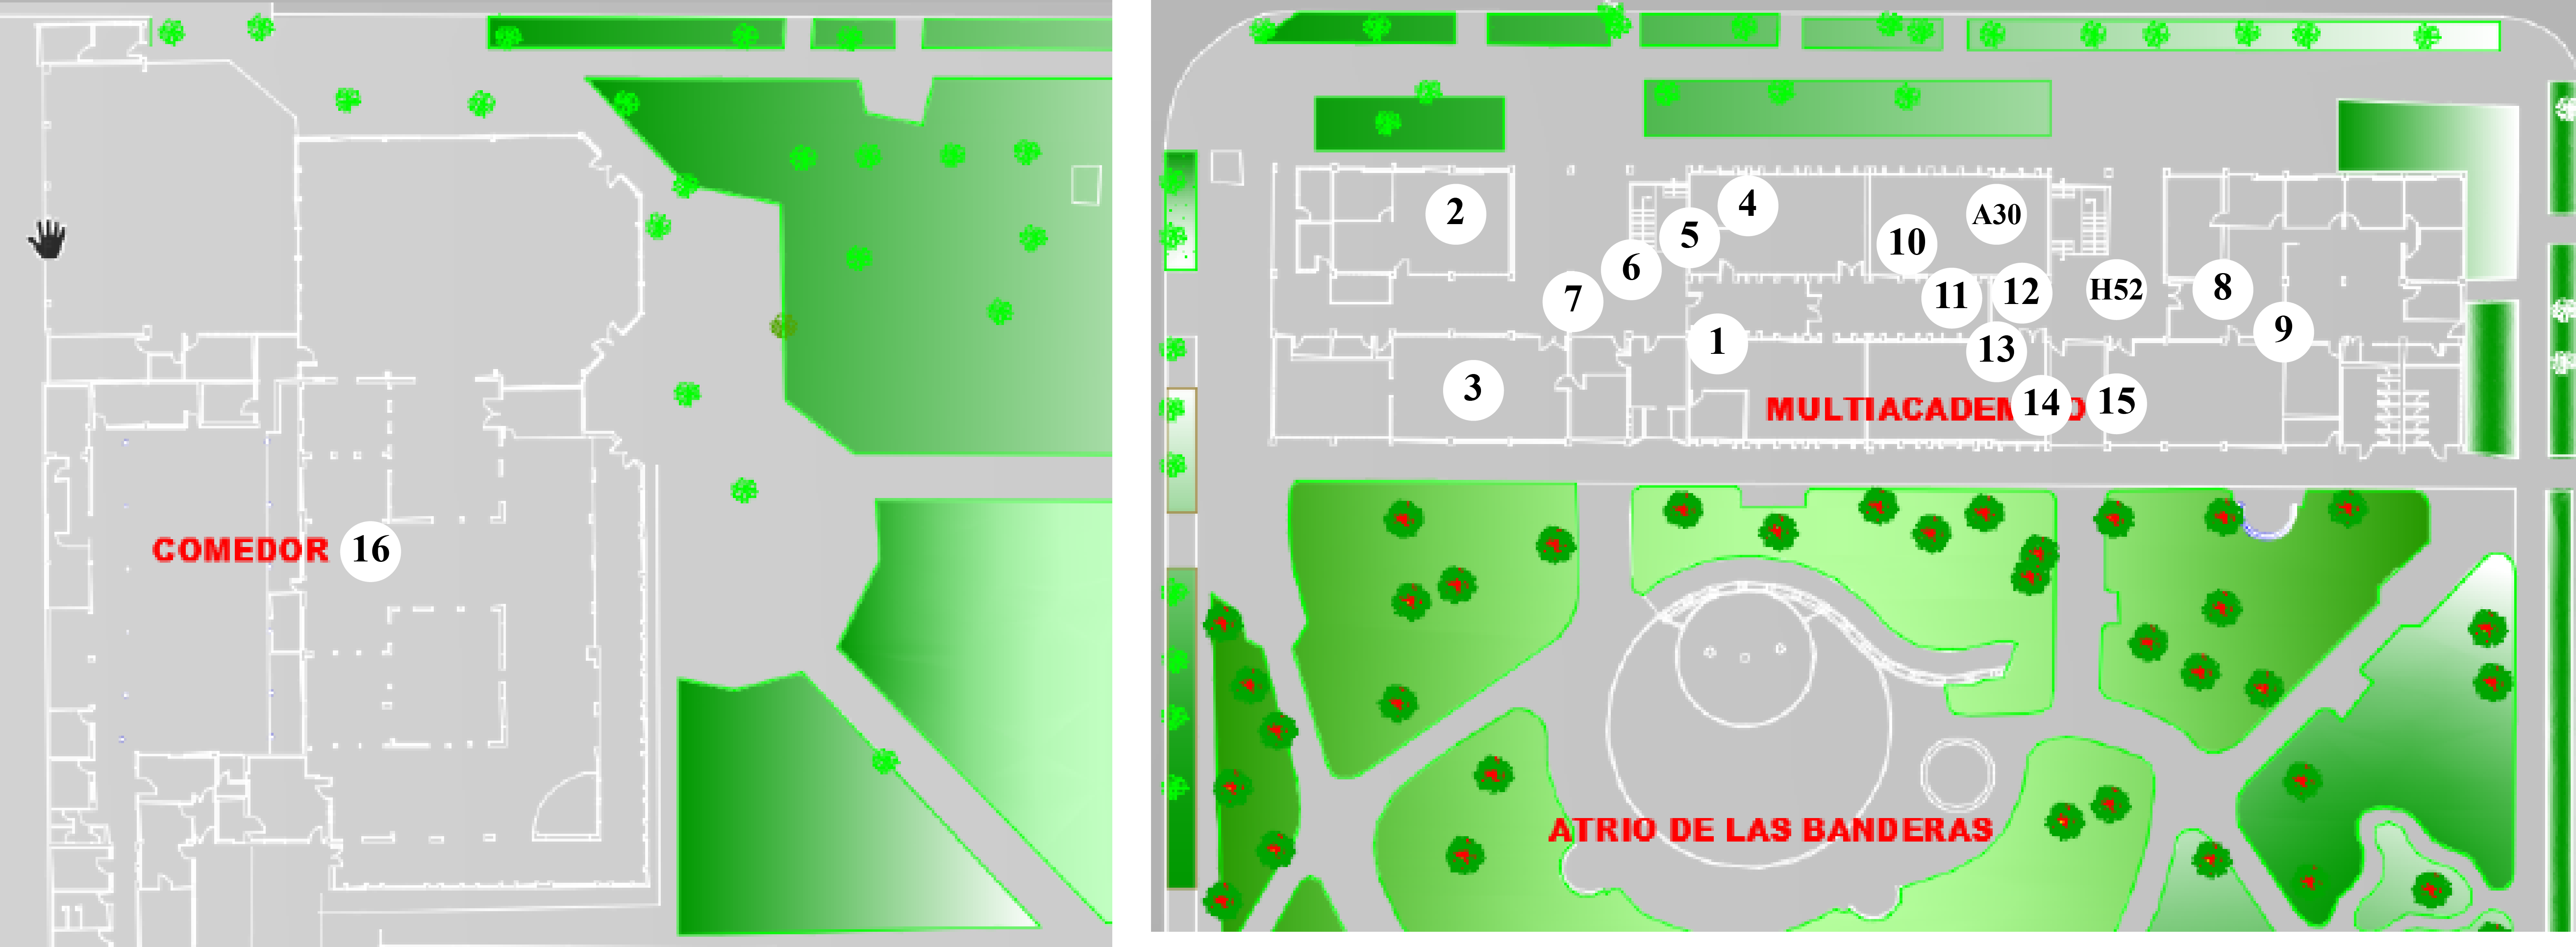
\includegraphics[width=0.9\textwidth]{multiacademico}
   \caption{Multiacademico - UMSS}
   \label{fig:multiacademico}
   \caption*{Fuente: Departamento Infraestructura - UMSS}
 \end{center}
\end{figure}

\newpage

\LTXtable{0.8\textwidth}{facultades/multiacademico}
% % \begin{table}
%   \begin{center}
    \begin{longtable}{ c  X }
      \toprule
        \textbf{Punto} &
        \textbf{Detalle}\\

      \midrule
      \endhead

\textbf{1}
&
PB - Unidad de Archivos Diplomas y Títulos (Legalizaciones)
\\

\textbf{2}
&
PB - Entrega de Diplomas
\\

\textbf{3}
&
PB - Departamento de Registros e Inscripciones
\\

\textbf{4}
&
1{\tiny er} Piso - DPA, Direccion de Planificacion Academica
\\


\textbf{5}
&
2{\tiny do} Piso - Planificación del Territorio y del Medio Ambiente
\\


\textbf{6}
&
3{\tiny er} Piso - Sala Consejo Universitario, Vice-Rectorado, PTAANG (Programa de Titulación de Alumnos Antiguos No Graduados)
\\


\textbf{7}
&
4{\tiny to} Piso - Jefatura de Personal Administrativo
\\


  \textbf{8}
  &
  PB - DISU (Dirección de Interacción Social Universitaria)
  \\

% \textbf{9}
% &
% PB - Aula 228 y Aula 229
% \\

\textbf{9}
&
1{\tiny er} Piso - Aula Internado Psicologia, Brigadas Universitarias de Salud
\\


\textbf{10}
&
1{\tiny er} Piso - PROTICS (Programa de Tecnologias de Informacion y Comunicacion Aplicadas a la Educación)
\\

% \textbf{6}
% &
% 1{\tiny er} Piso - Aulas: 233, 234, 237, 240, 241, 243
% \\

\textbf{11}
&
2{\tiny do} Piso - PROGEO (Programa de Geografía), Instituto de Investigaciones de Arquitectura, PROMESHA, Biblioteca IIACH
\\

\textbf{12}
&
2{\tiny do} Piso - CLAS (Centro de Levantamientos aeroespaciales y aplicaciones SIG para el desarrollo sostenible de los recursos naturales)
\\


\textbf{13}
&
3{\tiny er} Piso - DICyT (Dirección de Investigación Científica y Tecnológica)
\\



\textbf{14}
&
3{\tiny er} Piso - DUBE (Dirección Universitaria de Bienestar Estudiantil)
\\


\textbf{15}
&
4{\tiny to} Piso - DUEA (Dirección Universitaria de Evaluacion y Acreditacion - UMSS)
\\

\textbf{16}
&
Comedor Universitario
\\


\textbf{M17}
&
Caja Central UMSS (ver en el mapa de la Fac. Tecnologia, figura \ref{fig:fac_tecno})
\\


\textbf{M18}
&
Ofinica Almacenes Adquisiciones (ver en el mapa de la Fac. Tecnologia, figura \ref{fig:fac_tecno})
\\

      \bottomrule
      \caption{Locaciones del Multiacademico}
      \label{tab:lugares_multiacademico}
    \end{longtable}
%   \end{center}
% \end{table}


\newpage

\section{Complejo Deportivo}
\label{sec:canchas}

También podemos encontrar dentro del campus Universitario, el complejo deportivo cuyo mapa se puede ver en la figura \ref{fig:canchas} y el correspondiente detalle en la tabla \ref{tab:canchas}

\begin{figure}[H]
 \begin{center}
   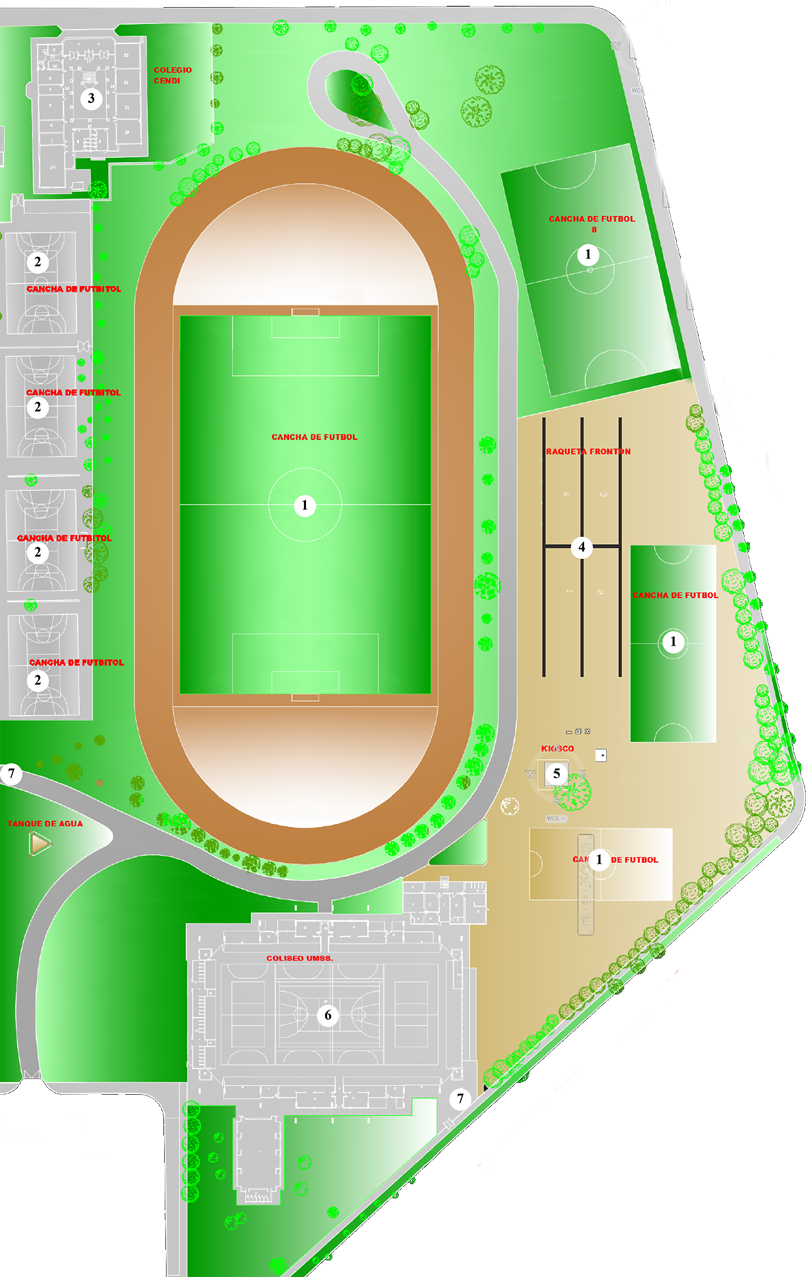
\includegraphics[width=0.5\textwidth]{canchas}
   \caption{Complejo Deportivo - UMSS}
   \label{fig:canchas}
   \caption*{Fuente: Departamento Infraestructura - UMSS}
 \end{center}
\end{figure}


\LTXtable{0.50\textwidth}{facultades/canchas}


\section{Facultades fuera del campus Universitario}
\label{sec:Facultades fuera del campus Universitario}

Las siguientes facultades no se hallan dentro del campus Universitario ``Las Cuadras'' por lo que escapan del alcance del presente proyecto de grado, pero se las nombrara para el conocimiento del lector.

\begin{description}
  \item[FACSO:] La Facultad de Ciencias Sociales o ``SOCIOLOGÍA'' está ubicada Nataniel Aguirre No. S 0360 entre Santivañez y Jordán, también conocida como ``Campus Sociología''.
  \item[FByF:] Facultad de Ciencias Farmacéuticas y Bioquímicas ubicada sobre Av. Aniceto Arce frente Parque La Torre.
  \item[FCAPFyV:] Facultad de Ciencias Agrícolas, Pecuarias, Forestales y Veterinarias
  Facultad de Ciencias Agrícolas, Pecuarias y Forestales ``Martin Cardenas'' (FCAPyP) ubicada en la Avenida Petrolera Km 5.
  \item[ODONTOLOGÍA:] Facultad de Odontología ubicada dentro el ``Campus Salud'', Calle Venezuela y Av. Oquendo.
  \item[MEDICINA:] Facultad de Medicina ubicada en el ``Campus Salud'', Av. Aurelio Melean 379.
  \item[FPVA:] Facultad Politecnica del Valle Alto ubicada en la Av. Mayor Rocha Provincia Punata.
  \item[FDRyT:] Facultad de Desarrollo Rural y Territorial  ubicada en la Av. Petrolera Km 5.5 carretera antigua a Santa Cruz.

\end{description}

% \item  - Facultad de Ciencias Sociales
% Dirección: Campus Sociología: Nataniel Aguirre No. S 0360 entre Santivañez y Jordán
% Teléfonos: 4502820 - 21 Fax: 4502821

% \item FByF - Facultad de Ciencias Farmacéuticas y Bioquímicas
% Dirección: Av. Aniceto Arce frente Parque La Torre
% Teléfonos: (591) (4) 420651 - (591) (4) 4250652


% FCAPFyV - Facultad de Ciencias Agrícolas, Pecuarias, Forestales y Veterinarias
%
% Dirección:
% Teléfonos: 4333808 - 4329666
%
% ODONTOLOGÍA - Facultad de Odontología
%
% Dirección: Campus Salud: C. Venezuela y Av. Oquendo
% Teléfonos: 4530307 - 4530314
% Fax. 4530314
%
% MEDICINA - Facultad de Medicina
%
% Dirección: Campus Salud: Av. Aurelio Melean 379
% Teléfonos: 4231508 - 4254910
%
% FPVA - Facultad Politecnica del Valle Alto
%
% Dirección: Av. Mayor Rocha Provincia Punata
% Teléfonos: (591)(4) 4577299
%
% FDRyT - Facultad de Desarrollo Rural y Territorial
%
% Dirección: Av. Petrolera Km 5.5 carretera antigua a Sta. Cruz
% Teléfonos: 4762387 - Telefax: 4761983
